
\begin{quote}
All numbers are generated by \texttt{eval/fidelity.py} from the full 836-image run with the shipped rule set (including the support depth gate, \S4.9) and are reproducible from \texttt{outputs/fidelity\_report.json}. The audit (\S4.4) predates the gate; \S4.9 reports the gate's effect on the audited samples.
\end{quote}

This chapter answers RQ1. It sets the evaluation protocol (\S4.1), reports the headline recall against every human label (\S4.2) with restricted precision (\S4.3) and an audited true-precision estimate (\S4.4), decomposes the hardest predicate pair per annotator (\S4.5), costs the residual human effort (\S4.7), and closes with the audit-driven rule repairs (\S4.9), a diagnosis of every remaining miss (\S4.10), the fully-automatic deployment mode (\S4.11), a video demonstration (\S4.12), the independent validation study (\S4.13), and a reliability test that uses the images' origin as consecutive frames of one robot capture to ask whether the labels survive the camera moving (\S4.14).

\section{Protocol}

RQ1 asks whether the automatic labels reach a quality comparable to human annotation. Two properties of the ground truth shape the protocol. First, the human annotations are \textbf{sparse}: 8,790 of 84,880 ordered object pairs (\textasciitilde{}10\%) carry a human label, so an automatic label absent from the gold is not necessarily wrong, and raw precision against the gold systematically undercounts. Second, annotator behaviour is \textbf{uneven} (Chapter 3 measured this for \texttt{near}; \S4.5 adds a second case), so agreement is reported per annotator group as well as pooled.

The evaluation therefore uses: (1) per-predicate \textbf{recall of the human triplets} as the primary metric, consistent with the recall-based convention of the source paper; (2) precision/recall/F1 \textbf{restricted to human-annotated pairs}; (3) a \textbf{manual audit} of a stratified sample of the tool's extra predictions, giving an unbiased estimate of true precision; (4) per-type \textbf{flag rates}, costing the human-in-the-loop claim; and (5) three baselines: random predicate, majority predicate, and \textbf{box-only geometry} (box centres, no masks, no depth). Object boxes and classes are ground truth throughout (the PredCls setting), so box IoU agreement is not applicable; detector-in-the-loop results appear with the ablations. Thresholds were fitted only on annotator groups 0--5; groups 6--8 are held out. A group is also a contiguous block of the underlying capture, so that split holds out an unseen object arrangement as well as an unseen annotator; \S4.14 establishes this and discusses what it qualifies.

\section{Headline: recall of the human triplets}

\begin{center}
\small
\begin{longtable}{lrrrrrr}
\caption{Per-predicate recall of the human triplets, pooled and on held-out annotators, against three baselines.}\\
\hline
Predicate & Gold & Ours & Ours (held-out) & Random & Majority & Box-only \\
\hline
\endfirsthead
\hline
Predicate & Gold & Ours & Ours (held-out) & Random & Majority & Box-only \\
\hline
\endhead
on & 1465 & 0.88 & 0.92 & 0.13 & 0.00 & 0.84 \\
under & 1001 & 0.81 & 0.92 & 0.16 & 0.00 & 0.77 \\
to the left of & 972 & 0.97 & 0.95 & 0.13 & 0.00 & 0.97 \\
to the right of & 1174 & 0.98 & 0.99 & 0.13 & 0.00 & 0.99 \\
in front of & 2013 & 0.64 & 0.20 & 0.13 & 1.00* & 0.00 \\
behind & 1584 & 0.66 & 0.35 & 0.16 & 0.00 & 0.00 \\
near & 717 & 1.00* & 1.00 & 0.16 & 0.00 & 0.87 \\
\textbf{mean} & 8,926 & \textbf{0.85} & \textbf{0.76} & 0.14 & 0.14 & 0.63 \\
\hline
\end{longtable}
\end{center}

\textbackslash{}\textit{ the majority baseline emits "in front of" everywhere, trivially recalling that class and nothing else. The near cell rounds 715/717 = 0.997 (\S4.9). The held-out front/behind cells (0.20/0.35) are dominated by two held-out annotator groups that labelled the pair with the }opposite direction convention*; \S4.5 decomposes this, and convention-aligned depth recall is 0.84.

These recalls are computed over every human triplet in the dataset, so they are population values rather than estimates from a sample. The question a reader still has is whether another batch from the same process would give the same numbers, and that is answered by a cluster bootstrap over images (\texttt{eval/uncertainty.py}; 2,000 resamples, whole images resampled with replacement so that triplets sharing a scene, a depth map and an annotator stay together). The 95\% intervals are narrow for the predicates the tool handles well, on 0.879 (0.863--0.895), left 0.965 (0.954--0.975), right 0.985 (0.977--0.992), near 0.997 (0.993--1.000), and materially wider for the depth pair, in front of 0.640 (0.602--0.678) and behind 0.655 (0.615--0.692), which is the expected signature of a predicate whose outcome depends on scene composition rather than on a stable rule. The held-out intervals appear with the per-annotator analysis in \S4.6.

Three observations. \textbf{(i)} The tool recovers 81\% of all human triplets (7,237 of 8,926; mean per-predicate recall 0.85, and 0.76 on annotators whose data never influenced any threshold), against 14\% for both trivial baselines. \textbf{(ii)} The box-only baseline matches the full pipeline on every box-computable predicate; the segmentation masks contribute essentially nothing to on/under/left/right/near recall (mask centroids $\approx$ box centres). The full pipeline's advantage is confined to the depth predicates (0.64/0.66 vs 0.00), and even the ground-plane fallback, a pure box cue, needs masks to fire, because its elevation guard is the mask-contact evidence (\S4.9). This raises a design question the ablations pursue: is SAM2 needed at all, or is its real contribution depth \textit{sampling} quality? \textbf{(iii)} The held-out column is higher than the pooled column for on/under/near and far lower for front/behind, which is an annotator-behaviour signature in both cases. For front/behind the cause is the convention inversion unpacked in \S4.5; for on/under it is direction-usage asymmetry: several groups label only one direction of a support pair (group\_2 records 188 \textit{on} and zero \textit{under}; group\_8 only \textit{under}), and the held-out groups' support labels happen to be canonical stackings the rules recover at 0.95--1.00. Gold totals here are 8,926 rather than 8,928 because two stray annotation files without matching images are excluded (Chapter 3).

\begin{figure}[htbp]
\centering
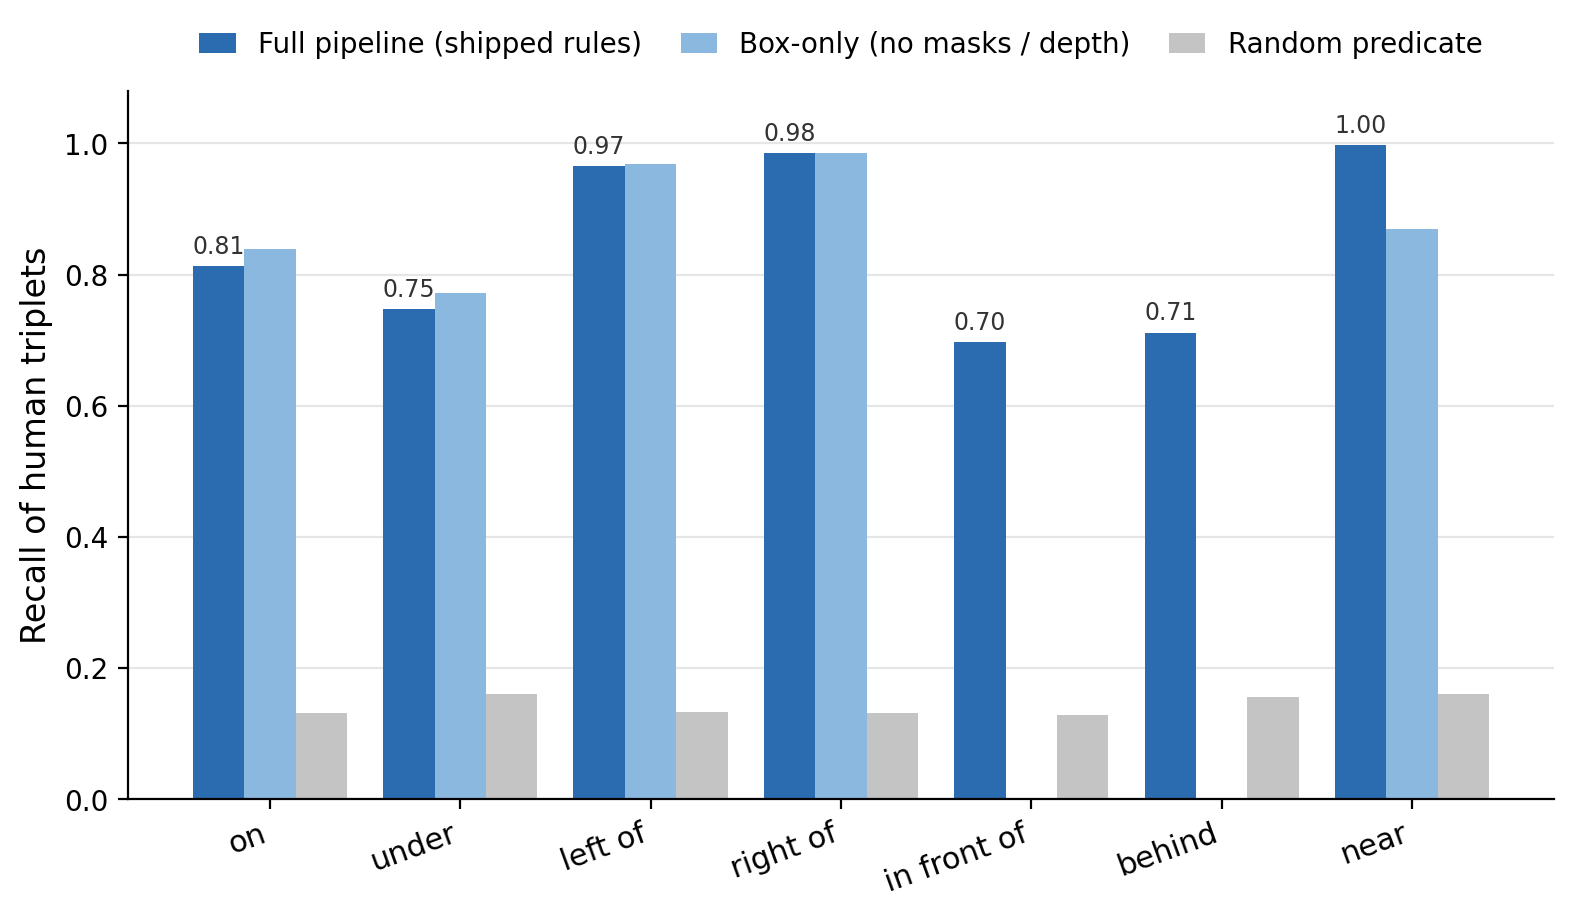
\includegraphics[width=0.95\textwidth]{figures/rq1-recall.png}
\caption{Recall of the human triplets per predicate: the full pipeline against a box-only ablation and a random baseline. Front and behind have no box-only bar because that ablation cannot compute depth.}
\label{fig:rq1-recall}
\end{figure}

\section{Precision on the annotated pairs}

\begin{center}
\small
\begin{longtable}{lrrrr}
\caption{Precision, recall and F1 restricted to the human-annotated pairs.}\\
\hline
Predicate & P & R & F1 & support \\
\hline
\endfirsthead
\hline
Predicate & P & R & F1 & support \\
\hline
\endhead
on & 0.88 & 0.88 & 0.88 & 1465 \\
under & 0.84 & 0.81 & 0.83 & 1001 \\
to the left of & 0.35 & 0.96 & 0.51 & 972 \\
to the right of & 0.42 & 0.98 & 0.59 & 1174 \\
in front of & 0.43 & 0.64 & 0.51 & 2013 \\
behind & 0.36 & 0.66 & 0.46 & 1584 \\
near & 0.12 & 1.00 & 0.21 & 717 \\
\hline
\end{longtable}
\end{center}

Restricted to the 8,790 human-annotated ordered pairs, precision is bounded below by construction: on an annotated pair the human typically recorded one or two relations, while several are geometrically true at once (a pair can be near, left-of and in-front-of simultaneously). The \texttt{near} row is the extreme case, since the tool emits \texttt{near} densely wherever the fitted gap threshold holds while only 3 of 9 annotator groups ever used the label, and it is exactly why the protocol includes the audit (\S4.4) rather than reading these columns at face value.

\subsection{Confusion: what the tool said when it missed}

For each human triplet the tool failed to recover, the labels it \textit{did} emit on that pair identify the failure mode directly:

\begin{center}
\small
\begin{longtable}{lrr}
\caption{For each missed human triplet, the predicates the tool emitted instead.}\\
\hline
Gold predicate & Missed & Most frequent co-emissions on missed pairs \\
\hline
\endfirsthead
\hline
Gold predicate & Missed & Most frequent co-emissions on missed pairs \\
\hline
\endhead
on & 177/1465 & near (177), behind (155): support demoted to proximity/depth \\
under & 187/1001 & in front of (167), near (166) \\
to the left of & 34/972 & near (33), to the right of (24): flips at the centre band \\
to the right of & 18/1174 & to the left of (16) \\
in front of & 725/2013 & near (572), behind (422), to the left of (261) \\
behind & 546/1584 & near (421), in front of (353) \\
near & 2/717 & on (2): the contact-exclusion boundary \\
\hline
\end{longtable}
\end{center}

Two structural signatures stand out. Missed front/behind pairs carrying the \textit{opposite} direction (422 + 353) are almost entirely the convention-inverted groups of \S4.5, and their count \textit{rose} with the ground-plane fallback, because pairs the tool used to abstain on are now committed in the direction those groups invert. And the two remaining missed \texttt{near} pairs carry \texttt{on}/\texttt{under}: the two rules disputing the contact boundary, the same support-rule frontier the audit (\S4.4) identifies from the precision side.

\begin{figure}[htbp]
\centering
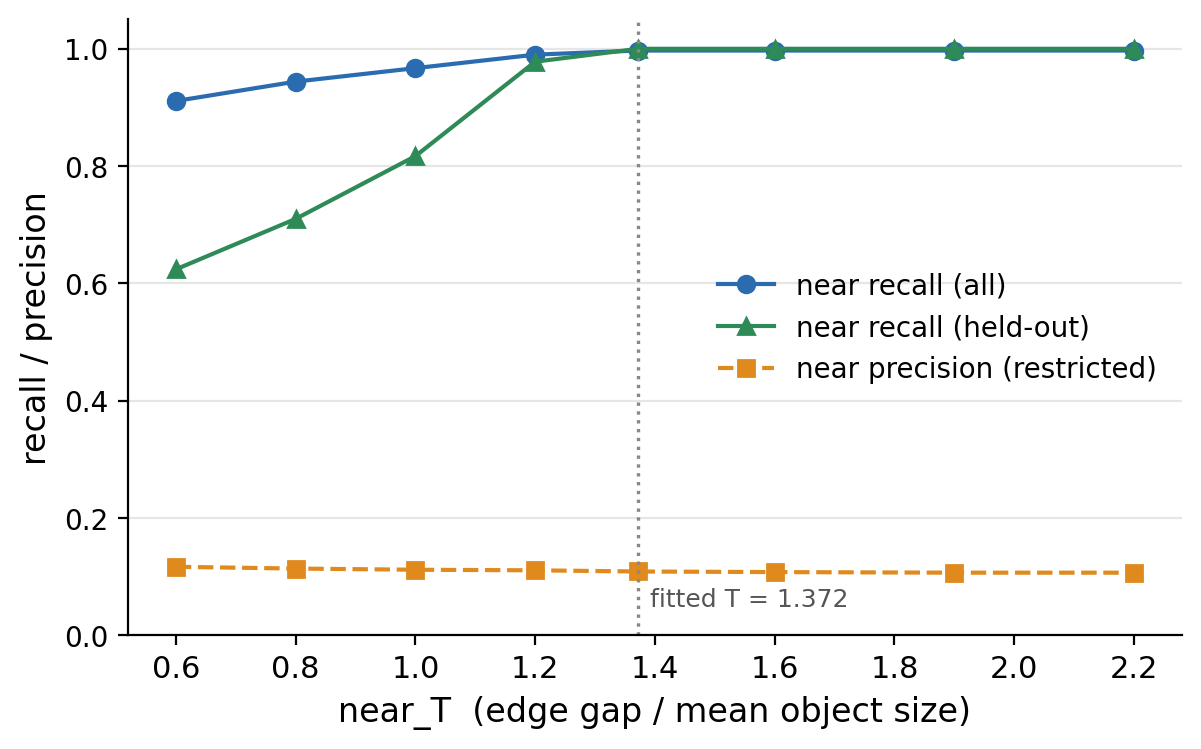
\includegraphics[width=0.95\textwidth]{figures/near-T-sweep.png}
\caption{Fitting the \texttt{near} threshold. Recall against all annotators and against the held-out annotator, with restricted precision. The fitted value is the tightest threshold at the plateau.}
\label{fig:near-T-sweep}
\end{figure}

\section{Manual audit of extra predictions (true-precision estimate)}

105 extra predictions (15 per predicate, seeded stratified sample) were rendered with subject/object boxes and manually verdicted, using a conservative rule under which any case not clearly true was marked wrong (\texttt{outputs/audit/audit\_sheet.csv}; verdicts to be independently spot-checked). This audit was run against the \textit{pre-gate box rule} and is reported as found because it motivated the support-rule repairs; \S4.9 re-audits the shipped rules (support precision \textasciitilde{}0.27 $\rightarrow$ \textasciitilde{}0.9), so the support rows below describe a fixed failure, not the final tool.

\begin{center}
\small
\begin{longtable}{lrrr}
\caption{Manual audit of a stratified sample of extra predictions, with Wilson intervals.}\\
\hline
Predicate & Correct / n & Precision est. & Wilson 95\% CI \\
\hline
\endfirsthead
\hline
Predicate & Correct / n & Precision est. & Wilson 95\% CI \\
\hline
\endhead
on & 1 / 15 & 0.07 & [0.01, 0.30] \\
under & 3 / 15 & 0.20 & [0.07, 0.45] \\
to the left of & 15 / 15 & 1.00 & [0.80, 1.00] \\
to the right of & 15 / 15 & 1.00 & [0.80, 1.00] \\
in front of & 15 / 15 & 1.00 & [0.80, 1.00] \\
behind & 15 / 15 & 1.00 & [0.80, 1.00] \\
near & 15 / 15 & 1.00 & [0.80, 1.00] \\
\hline
\end{longtable}
\end{center}

The audit splits the predicates cleanly in two. For the lateral, depth and proximity predicates, \textbf{every sampled extra prediction was correct}: the low restricted precision in \S4.3 is an artefact of sparse human labelling, exactly as the protocol anticipated, and the tool's dense labels on unannotated pairs are (within the sample's confidence bounds) trustworthy. For the support pair the picture inverts: extra \texttt{on}/\texttt{under} labels are mostly \textbf{false fires}. The box-adjacency test triggers on objects that merely project next to each other in clusters (a book \textit{behind} a bottle, a cube on the floor with a remote lying in front). Combined with \S4.2's containment misses, both error directions of the support rule point to the same repair, a mask-contact test instead of box adjacency, which the ablations evaluate. Two honest caveats: the sample is 15 per predicate, so per-predicate estimates carry wide intervals; and depth verdicts on near-coincident objects were occasionally marginal (noted in the sheet).

\section{The front/behind decomposition: a second measured annotation defect}

\begin{center}
\small
\begin{longtable}{lrrrrrr}
\caption{Front/behind by annotator group: emission rate, agreement where the tool commits, and the effect of aligning the direction convention.}\\
\hline
Group & Gold & Emit rate & Agreement when committed & Convention & Raw recall & Aligned recall \\
\hline
\endfirsthead
\hline
Group & Gold & Emit rate & Agreement when committed & Convention & Raw recall & Aligned recall \\
\hline
\endhead
group\_0 & 724 & 0.92 & 0.95 & same & 0.88 & 0.88 \\
group\_1 & 639 & 0.98 & 1.00 & same & 0.98 & 0.98 \\
group\_2 & 351 & 0.58 & 1.00 & same & 0.58 & 0.58 \\
group\_3 & 258 & 0.54 & 0.98 & same & 0.53 & 0.53 \\
group\_4 & 65 & 1.00 & 0.57 & same & 0.57 & 0.57 \\
group\_5 & 371 & 1.00 & 0.99 & same & 0.98 & 0.98 \\
group\_6 & 415 & 0.98 & \textbf{0.05} & \textbf{inverted} & 0.05 & 0.93 \\
group\_7 & 330 & 0.90 & 1.00 & same & 0.90 & 0.90 \\
group\_8 & 444 & 0.73 & \textbf{0.02} & \textbf{inverted} & 0.01 & 0.71 \\
\textbf{overall} & 3597 &  &  &  & \textbf{0.65} & \textbf{0.84} \\
\hline
\end{longtable}
\end{center}

(The table reports the shipped cascade, depth ordering plus the ground-plane fallback of \S4.9; the fallback roughly doubled the emit rates of the abstention-heavy groups 2 and 3.) The pooled 0.65 decomposes into three distinct causes:

\begin{enumerate}
\item \textbf{Direction agreement is near-perfect where the tool commits.} For six of
the eight groups with meaningful counts, agreement \textit{when a direction is emitted} is 0.95--1.00. Genuine depth-ordering errors are rare.
\item \textbf{Two annotator groups used the inverted convention.} Groups 6 and 8 agree
with the committed direction 2--5\% of the time; flipping their labels recovers 0.93/0.71. After the \texttt{near} findings, this is a \textit{second}, independent, measured annotation-consistency defect in the dataset: the direction convention for in front of/behind was not applied uniformly across annotators. This is the reference-frame ambiguity RoboSpatial formalises (\S2.5) observed in the wild: with no frame declared in the guidance, two annotator teams resolved it in opposite directions. (Aligned overall recall: 0.84. Alignment uses one disclosed bit per group, the majority direction of that group's own labels.)
\item \textbf{The remaining gap is abstention, not error.} Groups 2 and 3 agree with
the tool almost perfectly when it commits, but their scenes place object pairs inside the \texttt{depth\_eps} ambiguity band \textit{and} out of the ground-plane fallback's reach (elevated objects, near-tied bottom edges), so the tool abstains (emit rates 0.58 and 0.54, roughly doubled by the fallback from 0.30 and 0.08). The \texttt{depth\_eps} and \texttt{plane\_band} sweeps in the ablations trade this abstention against precision explicitly.
\end{enumerate}

\begin{figure}[htbp]
\centering
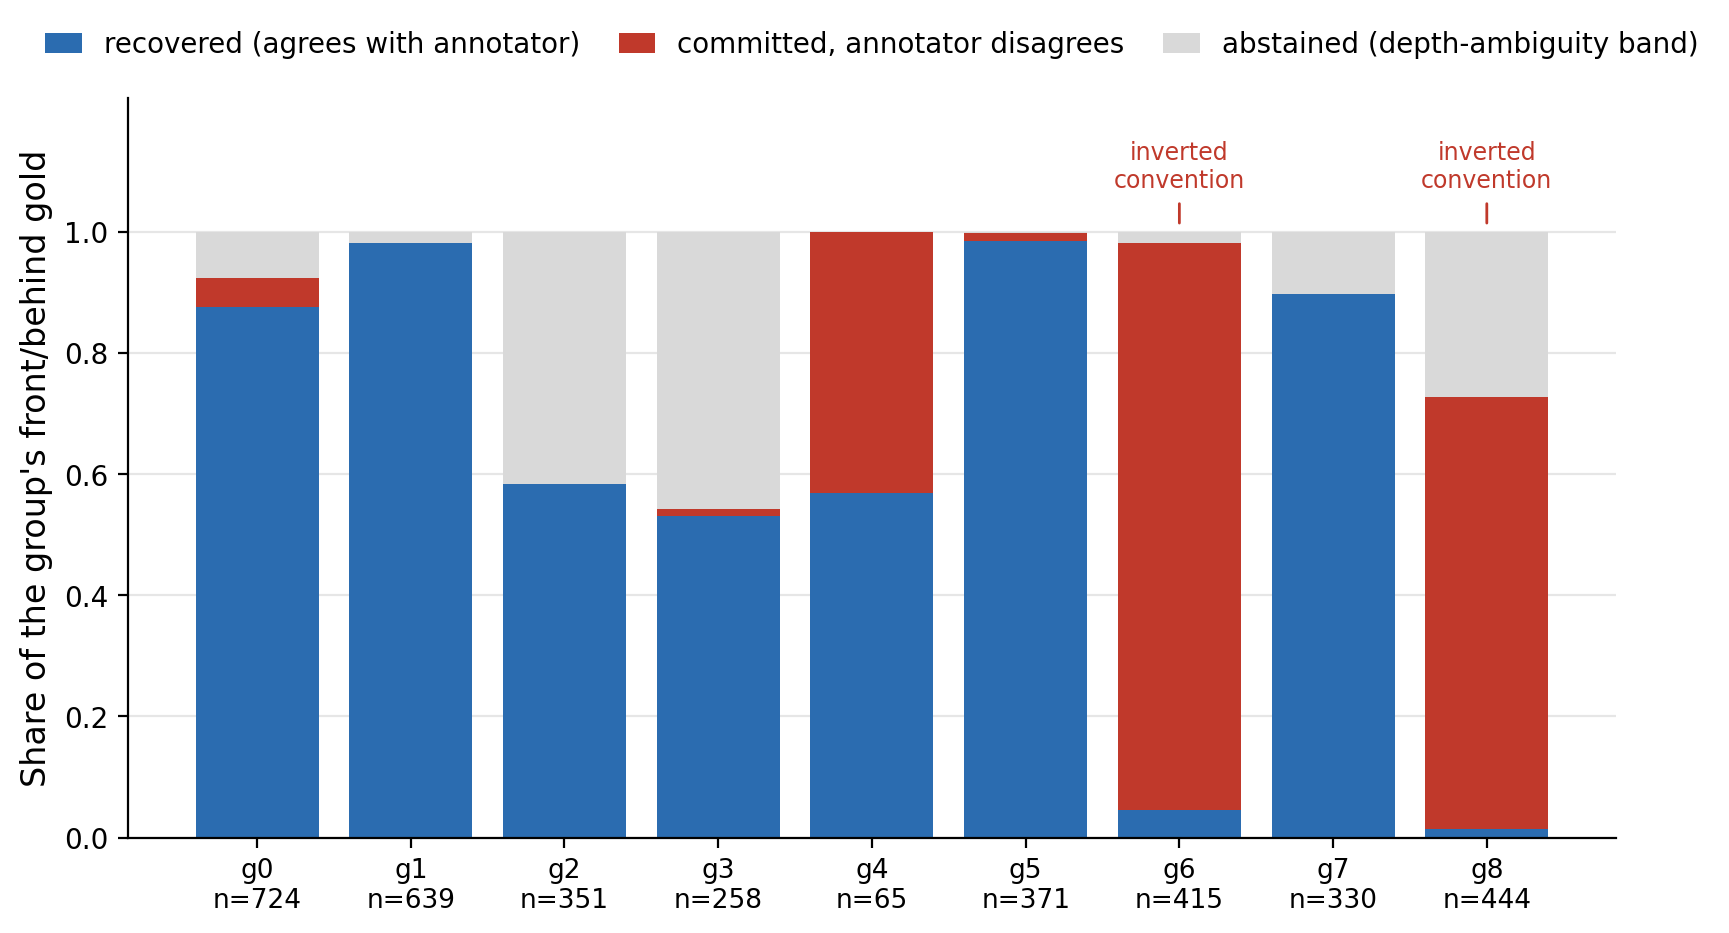
\includegraphics[width=0.95\textwidth]{figures/front-behind-decomposition.png}
\caption{Front/behind decomposed per annotator group: agreement where the tool commits, deliberate abstention, and the two groups that used the inverted direction convention.}
\label{fig:front-behind-decomposition}
\end{figure}

\section{The tenth annotator, and what the annotators would score against each other}

Per-group recall of each annotator's triplets (all predicates): group\_0 0.87 · group\_1 0.93 · group\_2 0.86 · group\_3 0.72 · group\_4 0.87 · group\_5 0.93 · group\_6 0.58 · group\_7 0.91 · group\_8 0.57. The dispersion is driven almost entirely by the two convention-inverted groups (6, 8): the tool agrees with the \textit{consistent} annotators at 0.72--0.93 (0.86--0.93 outside the abstention-heavy group 3).

On the held-out annotators specifically, the cluster-bootstrap intervals of \S4.2 are: on 0.922 (0.891--0.951), under 0.922 (0.879--0.960), left 0.953 (0.937--0.970), right 0.985 (0.974--0.996), near 1.000 (1.000--1.000), against in front of 0.197 (0.147--0.255) and behind 0.347 (0.281--0.417). Five of the seven predicates generalise to unseen annotators with intervals entirely above 0.87; the two depth predicates are separated from them by a gap far wider than the sampling uncertainty, which is what makes the convention explanation below a claim about the labels rather than about noise.

Reading those numbers as a quality verdict requires a yardstick the dataset does not supply: how well would two \textit{human} annotators agree with each other? The groups labelled disjoint image batches, so the quantity cannot be measured directly, and that absence is itself a finding about the dataset's construction. Two things can nevertheless be recovered by treating the automatic annotator as a fixed common reference (\texttt{eval/annotator\_agreement.py}).

\textbf{Annotator heterogeneity, measured without assumptions.} The tool is deterministic: it is literally the same labeller for every group, applying one definition. Any variation in its agreement across annotators is therefore variation in the \textit{annotators}. Across the seven consistent groups that variation spans 0.717 to 0.933, a spread of 0.216 (sd 0.068). Before any inference about human-human agreement, this alone establishes that the annotators are not interchangeable, and it puts a number on how far apart they are.

\textbf{Bounds on human-human agreement.} For any common reference, if annotator A agrees with it on a fraction p\_A of items and B on p\_B, their mutual agreement p\_AB obeys the Fréchet inequalities max(0, p\_A + p\_B − 1) $\leq$ p\_AB $\leq$ 1 − |p\_A − p\_B|. Averaged over all 21 pairs of consistent annotators, these place annotator-to-annotator agreement in \textbf{[0.74, 0.92]}. The tool's own mean agreement with those annotators, \textbf{0.869, lies inside that interval}. In other words, the automatic annotator agrees with the human annotators about as well as the evidence permits them to agree with each other. One assumption is required and is stated rather than buried: because the batches are disjoint, the bounds presume each annotator's agreement rate would carry over to another \textasciitilde{}100-image batch. The interval is therefore an estimate, not a measurement, and the independent validation study (\S4.13) is what tests the underlying precision claim without it.

\section{Flags: the honest human cost}

31.5\% of ordered pairs carry a flag: depth-ambiguous 19.3\% (down from 29.5\% before the ground-plane fallback, which resolved a third of the depth abstentions) and lateral-ambiguous 10.0\% are \textit{abstentions} (no label emitted; nothing to review), while the borderline-near band, 8.5\% of pairs, is the genuine review queue. At a conservative 3 seconds per queued pair this is $\approx$6 hours of review for the full dataset, versus the original nine-annotator manual pass. And it is optional, not required, for the fidelity reported above.

\subsection{The missing guidelines, confirmed at the source}

The annotation guidance the annotators worked from (confirmed from the SGDET-Annotate repository the supervisor indicated) consists of vocabulary lists only, object names and 19 relationship terms, with no operational definitions. Every annotator behaviour this chapter measures (the selective use of \texttt{near}, the inverted front/behind convention, one-directional support labelling) is the predictable consequence of labelling with undefined terms, the exact failure mode the annotator-disagreement literature documents across vision and language tasks (\S2.3). The geometric specification of Chapter 3 is therefore not a re-implementation of existing rules but the first operational definition of these predicates, and the fitted thresholds are exactly the "clear annotation guidelines" the source paper's future work requests.

\section{Answer to RQ1}

Automated annotation reaches human-comparable quality on six of seven predicates outright (0.81--1.00 recall of the human triplets; mean 0.85, with 0.76 on annotators no threshold ever saw), matches the human notion of \texttt{near} completely once the label's inconsistent usage is accounted for (0.997 pooled, 1.00 held-out at the fitted threshold), resolving the one predicate the source paper reports as failing for every model it benchmarks (\S2.2). On the depth pair, after the depth-plus-ground-plane cascade, it recalls 0.64/0.66 pooled and agrees with every consistently-labelled annotator 95--100\% of the time where it commits; aligned for the two inverted-convention groups, depth recall is 0.84. The remaining shortfall decomposes, in measured proportions, into calibrated abstention and that inverted convention. The audits bound true precision: \textasciitilde{}1.0 for the lateral and proximity predicates and for depth-decided front/behind, \textasciitilde{}0.9 for support after the contact rule, and \textasciitilde{}0.73 conservative for the ground-plane fallback's added commits (\S4.9). The tool's residual cost is the \textasciitilde{}8\% borderline review queue, and its labels are 20$\times$ denser than the human set.

\section{Shipped from the ablations}

Four rule changes came out of the audit-and-ablation loop; each is reported with its calibration, its held-out validation and its audit.

\subsection{The support depth-co-location gate}

The audit's support-precision failure has a geometric cause: on a floor plane, "farther" projects as "higher in the image", so a behind-pair produces the same 2D box signature as a stacked pair. The repair is a depth co-location condition on \texttt{on}/\texttt{under} (truly stacked objects share a camera distance), an instance of the reject-the-geometrically-impossible correction principle adapted from Open3D-VQA (Zhang et al., 2025; \S2.5), calibrated on the train groups (\texttt{on\_depth\_eps} = 0.06) and validated held-out (ablation A1): support F1 on never-seen annotators rises 0.58 $\rightarrow$ 0.71. Downstream effects on the headline table: support recall −2/−3 points, \texttt{on} restricted precision 0.57 $\rightarrow$ 0.73, 44\% fewer support emissions (of the 26 audited false positives, the gate removes 12 while keeping all 4 true positives), and, because fewer false contacts suppress fewer proximity labels, \texttt{near} recall rises 0.87 $\rightarrow$ 0.95 (held-out 1.00). Mean recall is unchanged at 0.79 with a substantially more trustworthy label set. The residual false fires are same-depth cluster neighbours, which depth cannot separate by construction; they are addressed next.

\subsection{The mask-contact rule}

The support signature that boxes cannot see, masks can: A rests on B iff the pixels directly below A's mask-bottom boundary belong to B (\texttt{src/contact.py}), which captures both stacking and the containment case, and rejects side-by-side neighbours. Calibrated on the train groups (\texttt{on\_contact\_min} = 0.60; the train-F1 plateau is flat from 0.60--0.80, so the choice is uncritical), ablation A5: support F1 on held-out annotators rises again, 0.71 $\rightarrow$ \textbf{0.87}, with \texttt{on} recall 0.82 $\rightarrow$ 0.88 and restricted precision 0.73 $\rightarrow$ 0.88 simultaneously, the rare change that improves both error directions at once, exactly as the failure gallery and audit predicted. Knock-on: \texttt{near} recall reaches \textbf{0.997 pooled (715/717; the two residual misses are contact-boundary cases, \S4.10) and 1.00 held-out} as the last contact-boundary suppressions disappear; headline mean recall 0.79 $\rightarrow$ \textbf{0.81}. The A4 sweep confirms the fitted threshold sits exactly at the recall plateau's knee: recall is flat from T = 1.372 upward while emissions keep growing, so the fitted value is the least-permissive point achieving maximal agreement. A 30-sample re-audit of the new support extras confirms the precision claim independently: extras correct rise from 1/15 and 3/15 (box rule) to \textbf{11/15 and 12/15}, an estimated true support precision of \textasciitilde{}0.27 $\rightarrow$ \textasciitilde{}0.9. The seven remaining wrong/uncertain extras have structure: a person \textit{holding} a remote fires contact (holding ≠ resting), one occluded bottle-behind-bottle pair, and three distant clusters too small to verdict confidently. The person-holding mode is closed by a \textbf{class-aware guard}: annotators never label person-support (0 of 2,466 gold support triplets involve a person on either side), so \texttt{on}/\texttt{under} are simply not evaluated for that class, removing \textasciitilde{}130 false emissions at no recall cost, since the person side carried no gold to recover.

\subsection{The ground-plane fallback}

The depth abstention band was the single largest miss cause, and most of it is resolvable without depth at all: two objects standing on the same floor are depth-ordered by pure projection. The nearer object's box bottom sits lower in the image, a pixel-precise cue exactly where relative depth is noisiest. The shipped rule fires only where the depth rule abstained, only when \textit{neither} object rests on another object by the tool's own contact evidence (an elevated object's box bottom locates its support, not itself), and only outside a small bottom-edge band (\texttt{plane\_band} = 0.005, calibrated on the train groups; ablation A7). On the train groups the fallback adds 386 committed directions at 0.91 agreement; on held-out group 7 it adds 54 and \textbf{every one agrees with the annotator}. Effect on the headline: front/behind recall 0.52/0.55 $\rightarrow$ \textbf{0.64/0.66} (aligned overall 0.67 $\rightarrow$ \textbf{0.84}), mean recall 0.81 $\rightarrow$ \textbf{0.85}, and the depth-ambiguous flag rate falls 29.5\% $\rightarrow$ 19.3\%. A seeded 15-sample audit of the fallback's \textit{extra} predictions (pairs no human labelled) estimates true precision conservatively at \textbf{11/15 $\approx$ 0.73}, and the four wrong/uncertain cases share one structure: an object resting on something the detector has no box for (a book on an unannotated case; a stacked-book pair whose contact fell below threshold), i.e. elevation the guard cannot see. That residual mode is documented, bounded, and exactly the undetected-support refinement the support audit already motivates.

\subsection{Follow-up refinements: one shipped, two declined}

The class-aware guard \textit{shipped}: annotators never label person-support (0 of 2,466 gold triplets), so support is no longer evaluated when either object is a person, removing \textasciitilde{}130 held-object emissions at zero recall cost and eliminating the person-holding audit mode by construction. Two further candidates were built, measured, and rejected on the evidence. (i) \textit{Guard-only surface detection} (zero-shot prompts for tables, cases and trays feeding the elevation guard; \texttt{scripts/run\_surface\_guard.py}) suppressed 6\% of the fallback's extra commits at a cost of 0.01 behind recall, but blocked none of the four audited failures, whose supports are either annotated-class objects with below-threshold contact (flat stacked books) or surfaces the detector missed; the machinery and its cache are retained as an ablation (\texttt{outputs/surface\_guard\_ablation/}). (ii) \textit{A larger depth model} (Depth Anything v2 Base, 4$\times$ the parameters) moved front/behind recall by +0.001/+0.002: the remaining depth ambiguity lives in the scenes, not in model capacity, and the Small variant's Apache licence is kept. Both null results bound where further engineering can and cannot help.

\subsection{Why a geometric cue, not a bigger depth model (ablation A8)}

It is worth asking whether the depth pair would improve simply by using a stronger depth network. It does not: swapping Depth Anything v2 Small for the 4$\times$ larger Base variant and re-running the whole dataset moves front/behind recall by +0.005 (0.636/0.652 $\rightarrow$ 0.641/0.656) and mean recall by +0.000. The depth-predicate limit is \textit{monocular ambiguity} (two objects at a similar camera distance are inseparable by any monocular model, regardless of its fidelity), not the network's quality. This is precisely why the fallback that worked is a geometric projection cue rather than a heavier perception model, and it justifies shipping the Small variant: identical accuracy, an Apache-2.0 licence, and half the VRAM.


\section{Failure gallery: every miss diagnosed}

Each missed human triplet is diagnosed automatically by re-checking the rule's individual conditions against the cached geometry and mask-contact maps (\texttt{scripts/make\_failure\_gallery.py}; rendered examples in \texttt{outputs/failure\_gallery/}). With the shipped rule set (1,689 misses):

\begin{center}
\small
\begin{longtable}{ll}
\caption{Diagnosed cause of every missed human triplet, by predicate.}\\
\hline
Predicate & Dominant causes (share of that predicate's misses) \\
\hline
\endfirsthead
\hline
Predicate & Dominant causes (share of that predicate's misses) \\
\hline
\endhead
in front of & abstained in ambiguity band 61\% · convention-inverted annotators 38\% · \textbf{genuine depth error 1\%} \\
behind & abstained 52\% · convention-inverted 42\% · \textbf{genuine depth error 5\%} \\
on & mask contact below threshold 58\% · depth-gate suppressed 40\% \\
under & contact below threshold 50\% · depth-gate suppressed 33\% · no contact measured (occlusion) 17\% \\
near & 2 remaining misses (contact boundary) \\
to the left/right of & centre flip 71--89\% · abstained 11--29\% (52 cases total) \\
\hline
\end{longtable}
\end{center}

Genuine depth-ordering errors remain 1--5\% of front/behind misses; the support misses are threshold/gate trades on real contact evidence rather than box-geometry artefacts; and \texttt{near} misses have all but vanished. The convention-inverted \textit{share} grew (38--42\%, from 28--32\%) not because those misses increased but because the ground-plane fallback shrank the abstention share around them; total misses fell from 2,107 to 1,689. Misses attributable to avoidable tool error across all seven predicates: \textasciitilde{}7\%.


\section{Detector-in-the-loop: full automation, attributed}

The deployment mode replaces ground-truth boxes with Grounding DINO (Liu et al., 2024) zero-shot detection (short-noun text prompts for the six classes; threshold 0.25, tuned in one disclosed iteration on a 20-image trial), then runs the identical SAM2 $\rightarrow$ depth $\rightarrow$ rules stack (\texttt{scripts/run\_sgdet.py}, scored by \texttt{eval/sgdet\_eval.py} with class-matched greedy IoU $\geq$ 0.5).

End-to-end triplet recall over all 836 images is \textbf{0.38} against the PredCls headline, and the decomposition attributes the gap exactly. Zero-shot detection recall spans 0.40 (cube) to 0.95 (human), and a triplet needs \textit{both} endpoints found. \textbf{Conditioned on both endpoints being detected, the relation layer scores 0.85 mean, matching its PredCls performance} (lateral 0.96/0.98, near 1.00, support 0.83/0.77; front/behind 0.69/0.70, computed before the ground-plane fallback shipped, so the conditional depth numbers are a floor; detectable pairs also skew towards well-separated objects). The gap is therefore entirely a detection problem, not a relations problem: the geometric rules are detector-agnostic.

Two honest notes. Zero-shot open-vocabulary detection is the worst-case detector, exactly the reach-versus-per-class-recall trade \S2.6 identifies, and it was used because the authors' trained YOLOv10m weights (0.93 mAP@50 in the source paper) were not available; with that detector the end-to-end gap would largely close. And the 20-image trial over-estimated detection quality (its scenes come from one annotator batch), a reminder that the full-set numbers are the ones that matter.

\section{Video demonstration}

Two short royalty-free stock clips (sources in Appendix A) were processed per frame by the deployment-mode stack of \S4.11 with open-vocabulary prompts, greedy IoU tracking for stable object identities, and a $\pm$2-frame temporal majority vote over each pair's predicates (\texttt{scripts/run\_video.py}; overlays and per-frame records in \texttt{outputs/video/}). The clips were chosen as complementary regimes: a \textbf{moving camera over a static desk scene} (clip 1, 99 processed frames), where relations should stay constant and any variation is measurement noise; and a \textbf{static overhead camera with moving hands} (clip 2, 79 frames), where relations genuinely change and smoothing must not erase the change.

Three observations. \textbf{(i) Relations are stable wherever identity is stable.} For object pairs co-visible in $\geq$20 frames, the emitted predicate persists at 0.90/0.94 mean across the two clips, with 81\% and 89\% of pair-predicates present in $\geq$90\% of their co-visible frames (\texttt{eval/video\_stability.py}, which derives these from the recorded per-frame files; co-visible means both track identities appear in that frame). The temporal vote is what separates the two clips: it lifts persistence from 0.896 to 0.902 on the static-scene clip and from 0.915 to 0.938 on the one with moving hands, which is the clip where per-frame detection actually churns. Frame-to-frame triplet agreement (Jaccard 0.89 for clip 1, 0.70 for clip 2) is dominated by zero-shot detection churn and, in clip 2, genuine hand motion; the dips in the stability trace align with the hands picking objects up. This mirrors \S4.11's attribution exactly: the variation is detection, not relations. \textbf{(ii) The rules transfer to objects they were never calibrated on}: the pen resting on the notepad and a wallet-and-photograph stack are labelled with the same contact evidence fitted on the dataset's six classes. \textbf{(iii) The camera-frame semantics are visible}: in the bird's-eye clip, in front of/behind re-maps to distance from the viewer's edge of the desk, the reference-frame dependence \S2.5 cites from RoboSpatial, demonstrated rather than asserted. The open-vocabulary quirks are equally visible and worth recording: content displayed \textit{on the laptop's screen} is detected as real objects, and items outside the prompt list snap to the nearest prompted class (an earbuds case becomes a \texttt{cup}).

This is a demonstration, not an experiment (no video ground truth exists), but it establishes that the annotator is video-ready at \textasciitilde{}2--3 s per frame, with SAM2's native mask propagation (it is a video model used here frame-wise) as the designed upgrade path for true temporal consistency.

\textbf{It is also the project's only out-of-domain evidence, and worth reading as such.} The clips share nothing with the dataset the rules were calibrated on: different scenes (an office desk and an overhead worktop, not a laboratory floor), a different camera and viewpoint, and objects drawn almost entirely from outside the six annotated classes (a monitor, keyboard, mouse, mug, spectacles, potted plants, a lamp, a notepad, a laptop, a cactus, a wallet, photographs, an earbuds case). No threshold was retuned: \texttt{near\_T}, the depth band, the contact fraction and the plane band are the values fitted on annotator groups 0--5 of the robot dataset. The support relations that emerge (a pen resting on a notepad, a wallet-and-photograph stack) are decided by the same mask-contact evidence, and the camera-frame semantics behave exactly as the design predicts when the viewpoint changes to bird's-eye.

The limits of that evidence should be equally clear: with no ground truth these are qualitative judgements over two clips, so they support the claim that the \textit{rules} carry to new object types and viewpoints, and they say nothing quantitative about accuracy in a new domain. A labelled cross-domain sample is the measurement this substitutes for, and it remains future work (\S7.6). What the clips do settle is that transfer is not blocked by the object vocabulary: the failures visible in them are detection failures (screen content detected as real objects, unprompted items snapping to the nearest prompted class), which is the same attribution \S4.11 makes for the dataset itself.

\begin{figure}[htbp]
\centering
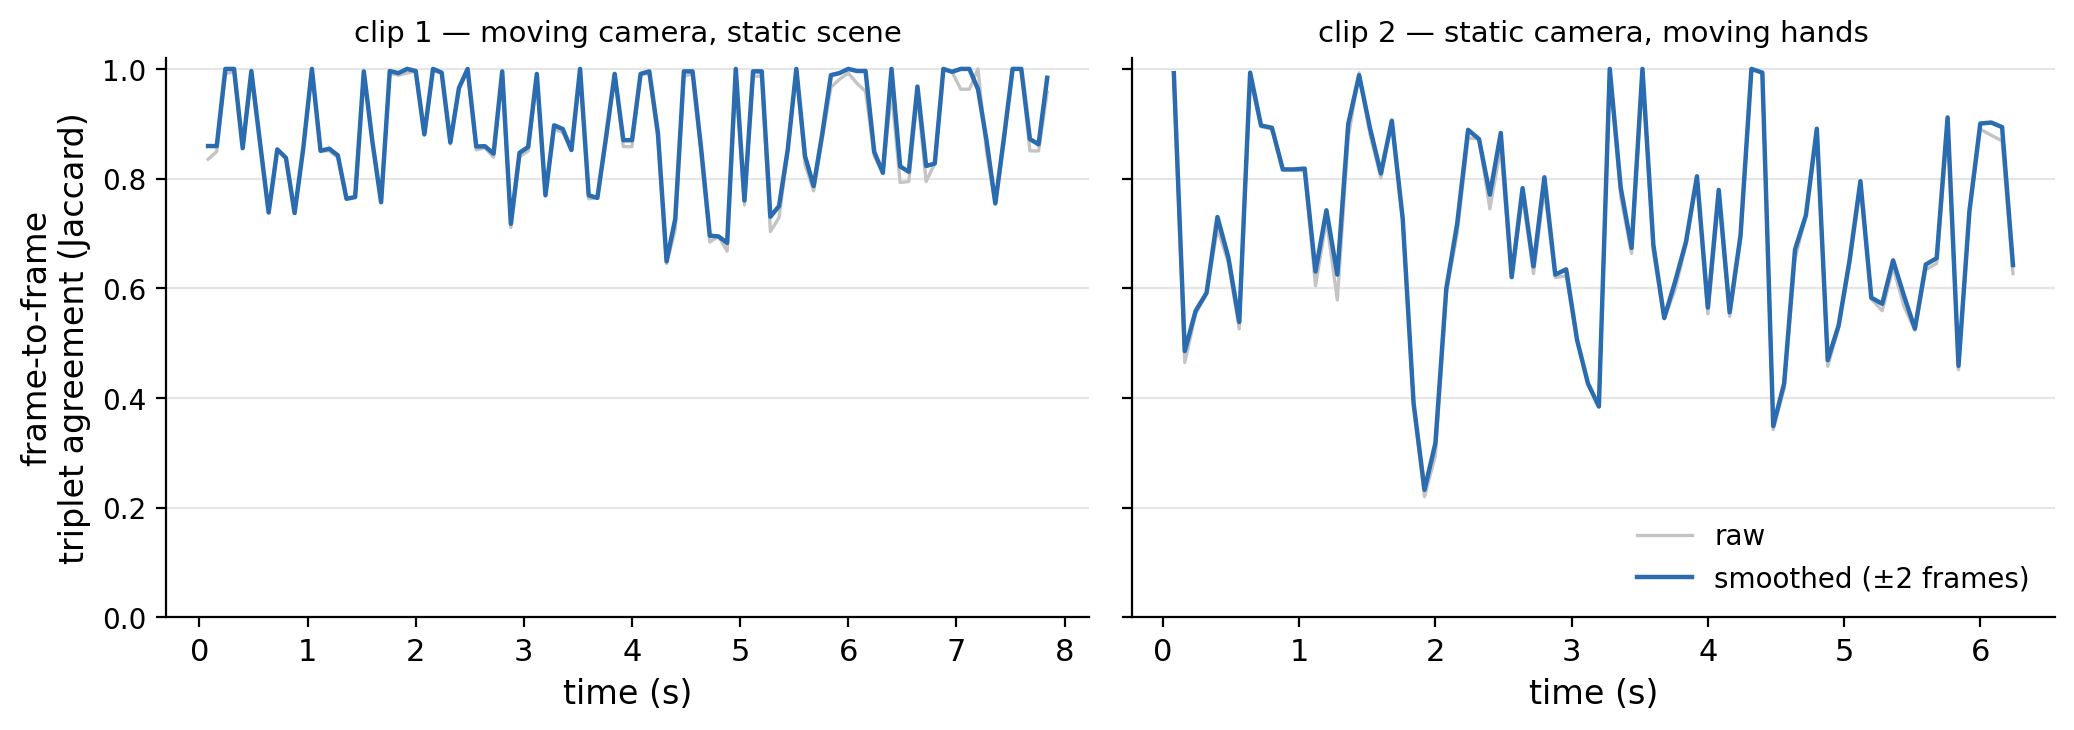
\includegraphics[width=0.95\textwidth]{figures/video-stability.png}
\caption{Frame-to-frame stability of the emitted triplets on the two demonstration clips, before and after temporal smoothing.}
\label{fig:video-stability}
\end{figure}

\section{Independent validation of the precision estimate}

The true-precision estimates of \S4.4 and \S4.9 have one methodological weakness that no amount of sampling fixes: they were verdicted by the author of the tool being evaluated. Conservative rules and published evidence mitigate the risk, but they do not remove it, and the honest description of those numbers is "author-verdicted". A separate study was therefore designed to re-estimate precision with judges who have no stake in the result.

\textbf{Protocol.} A stratified sample of 2,002 automatic labels (286 per predicate) is drawn from the tool's \textit{extra} predictions, meaning ordered pairs the human annotators never labelled, which is exactly the population with no ground truth to score against. Each claim is rendered as the source photograph with the subject outlined in red and the object in blue, and presented with a single sentence ("the book is on the box") to volunteers recruited by open link, who answer TRUE or WRONG / can't tell. The instructions restate the operational definitions of Chapter 3: camera-frame laterality, "in front of" as nearer the camera, support as physically resting rather than held, and an explicit instruction to answer WRONG when unsure, which reproduces the conservative rule used in the author's audits. Each browser receives a random identifier that prevents repeat judgements without identifying anybody, and faces are anonymised in every image (Chapter 8).

Coverage is stratified by what each analysis requires. An aggregate precision estimate needs only one judgement per claim, since the sample is random either way, so ordinary claims target a single rater. The 147 claims that also carry an author verdict target three raters each, because the crowd-versus-author comparison and the inter-rater reliability figure both need several independent judgements on the \textit{same} item; those claims are served first. The design therefore needs about 2,300 judgements rather than the 6,000 a uniform three-rater target would demand, and it fails gracefully: the author-comparison subset completes after roughly 30 participants, so that analysis survives a thin turnout while any further response widens the precision estimate.

\textbf{What it measures.} Three things the author-verdicted audits cannot. First, crowd precision per predicate with binomial confidence intervals, at a sample size two orders of magnitude larger than the n = 15 per predicate of \S4.4. Second, an author-bias check: the 147 items carrying the author's own verdicts are retained inside the pool, so crowd majority and author verdict can be compared directly by percentage agreement and Cohen's kappa (Cohen, 1960). Third, whether the \textit{task} is well posed at all, through crowd-internal reliability across raters (Krippendorff's alpha), which distinguishes "the tool is wrong" from "this claim is genuinely ambiguous", a distinction the annotator-disagreement literature insists on (\S2.3).

Scoring is fully specified in advance (\texttt{analysis/score\_votes.py}): ties resolve to WRONG, matching the audit protocol; reflex-speed responses and raters who disagree systematically with everyone else can be excluded by pre-declared filters. The instrument is complete and collection is under way; the results are reported at submission, and the limitation stated in \S7.4 stands until they are.

\section{Temporal redundancy and stability under viewpoint change}

The 884 released images are not independent photographs. Pixel-matching them against the 2,650-frame raw capture the supervising group later supplied identifies them exactly: they are frames 000000--000883 of one continuous walk, and each annotator group is a contiguous 100-frame block (\texttt{group\_0} = frames 0--99, \texttt{group\_1} = 100--199, and so on). This has two consequences, one methodological and one that yields a measurement the rest of the chapter cannot make.

\textbf{The methodological one first, because it qualifies earlier results.} A group is simultaneously an annotator identity \textit{and} a temporal block holding one arrangement of objects. The held-out split of \S4.1 is therefore held out by annotator \textit{and} by scene, not by annotator alone as described. The annotator reading survives, since a systematically inverted front/behind convention (\S4.5) and a \texttt{near} label used by three groups in nine (\S3.2) are properties of labelling behaviour, and no arrangement of furniture can produce them, but the held-out figures carry a domain shift alongside the annotator shift. The direction of that confound is favourable, in that 0.76 on held-out groups is generalisation to an unseen annotator \textit{and} an unseen arrangement, which is the harder of the two readings; it is recorded here because the design was described as one thing and the data supports a slightly stronger one.

\textbf{The measurement.} Because the frames are consecutive, a scene appears repeatedly from different viewpoints, and the pipeline's verdicts can be compared across those viewpoints without any human labels. The comparison is a reliability test of a kind sparse human annotation cannot supply: a relation determined by geometry should survive the camera moving, and one decided by a coin-toss at a decision boundary should not.

Frames were segmented by content drift (\S3.10) and each segment's predicates propagated from its keyframe to the remaining frames, matching objects by class and box overlap because object indices are not stable across frames: the annotators recorded different subsets of the scene from frame to frame, and \texttt{group\_0} alone contains 43 distinct object orderings (\texttt{eval/keyframe\_propagation.py}).

\textit{Segmentation.} At τ = 10 the full 2,650-frame sequence collapses to 892 segments, a 3.0$\times$ reduction; over the 884 released frames alone it gives 331 segments, 2.7$\times$. Scored on that released portion, where the eight layout changes are known, every one is recovered within five frames (boundary recall 1.00). Precision against those eight is low by construction and not a defect: viewpoint changes within a block are genuine content changes, merely finer-grained than the layout changes.

The comparison worth recording is with the standard alternative. Thresholding consecutive-frame differences, the basis of shot detection, does not merely perform worse here, it has no usable operating point at all. At a threshold of 15 grey levels it fires 13 times across the annotated frames and finds none of the eight; lowering it to 5 finds all eight but among 604 firings, a precision of 0.013, and lowering it further only adds firings. There is no setting at which the layout changes separate from the noise, because the per-step signal they produce is not larger than the noise; only the accumulated drift is.

\textit{Stability and cost.} The propagation runs over the 802 annotated frames that carry pair records, segmented within each group so no segment straddles two arrangements. At τ = 10 that yields 568 keyframes, leaving 234 frames whose predicates are propagated rather than computed, and 11,352 object pairs on which the two can be compared. (The compression here is lower than the 2.7$\times$ quoted above because these 802 frames are a subset of the sequence: consecutive members sit further apart in the original capture, so more drift accumulates between them.) The table below reports per predicate how often the keyframe's verdict matches what the pipeline computes on the frame directly, alongside recall of that frame's human triplets under propagation and under per-frame computation.

\begin{center}
\small
\begin{longtable}{lrrr}
\caption{Stability of each predicate across viewpoints of the same scene, with recall under keyframe propagation against per-frame computation.}\\
\hline
Predicate & Stability & Recall (propagated) & Recall (per frame) \\
\hline
\endfirsthead
\hline
Predicate & Stability & Recall (propagated) & Recall (per frame) \\
\hline
\endhead
on & 0.909 & 0.897 & 0.864 \\
under & 0.909 & 0.829 & 0.795 \\
to the left of & 0.989 & 0.959 & 0.966 \\
to the right of & 0.989 & 0.989 & 0.989 \\
in front of & 0.955 & 0.627 & 0.601 \\
behind & 0.955 & 0.601 & 0.613 \\
near & 0.966 & 1.000 & 1.000 \\
\textbf{Mean} & \textbf{0.953} & \textbf{0.843} & \textbf{0.832} \\
\hline
\end{longtable}
\end{center}

Skipping frames costs nothing measurable. Mean recall under propagation is 0.843 against 0.832 computed per frame, and the ordering holds at every threshold tested (0.879 against 0.861 at τ = 20, a 4.0$\times$ reduction). The small advantage is plausibly an artefact of the selection rule rather than a benefit of propagation: the segment representative is the frame nearest the segment mean, which on a moving camera is less likely to be caught mid-transition than an arbitrary frame.

\textbf{The finding that matters is in the first column, and it is not the one expected.} Front/behind was predicted to be the least stable predicate, on the assumption that its errors come from monocular depth noise near the decision boundary; noise of that kind should flip verdicts when the camera moves. It does not. Front/behind agrees with itself across viewpoint changes 0.955 of the time, above \texttt{on}/\texttt{under} at 0.909, and still 0.924 when the segmentation is coarsened to 89$\times$ compression, where segment members are substantially different views. A predicate whose recall against human labels is 0.60 while its agreement with itself across viewpoints is 0.96 is not making random errors. It is making the same call repeatedly and disagreeing with the annotators systematically.

That converges with two independent results. Ablation A8 (\S4.9) showed a depth model four times larger does not improve front/behind, which is what one expects if the limit is not depth resolution; and \S4.5 measured two annotator groups labelling the pair in the opposite direction, which is a disagreement about what the words mean. The viewpoint-stability figure adds the evidence those two could not: the tool's verdicts are reproducible under exactly the perturbation that would expose measurement noise. Monocular ambiguity remains a real bound on the predicate (\S9.3), but the gap between 0.64 and 1.00 on this dataset is dominated by definitional disagreement rather than by an unsteady depth estimate.

\textbf{Limits of this measurement.} Two, both restricting scope rather than direction. Stability is computed only on object pairs that could be matched between keyframe and frame, and those are pairs whose objects moved least in the image, which is plausibly the easier population; the figures are therefore an upper bound on stability over all pairs. And matched coverage falls sharply as segments grow, from 88.7\% of pairs at τ = 5 to 58.5\% at τ = 10 and 26.5\% at τ = 20, so aggressive compression leaves most pairs uncovered rather than mislabelled. The cause is box drift under camera motion rather than missing annotation: at τ = 20, 65\% of skipped frames carry an identical object count to their keyframe, and relaxing the overlap criterion from 0.5 to 0.1 cuts unmatched objects from 5.6 to 2.2 per frame. Carrying object identity with a tracker, which \texttt{scripts/run\_video.py} already does for video, rather than with per-frame overlap, is the change that would recover it, and it is a straightforward extension rather than a research question.

\section{Scale, measured rather than extrapolated}

Throughput and density elsewhere in this chapter are measured on the 836 annotated images, which leaves the claim that the method extends to new captures resting on an extrapolation. The 1,766 unannotated frames of the raw sequence (\S4.14, Appendix A) remove that gap: they are robot output nobody has labelled, from the same platform and laboratory but from later in the session, with arrangements and rooms the tool has never been shown.

No accuracy claim is available here, since there is no ground truth, and none is made. What the run establishes is operational, and there are three parts to it.

\textit{Cost.} Content-adaptive selection reduces 1,766 frames to 562 keyframes, 3.1$\times$. In deployment mode the pipeline sustains 3.33 s per frame on the RTX 2060 (1,080 frames per hour, JSON only; rendering an inspection overlay for every frame roughly doubles that). The keyframe pass therefore takes 31 minutes where annotating every frame would take 98.

\textit{Yield.} The run emits 185,242 triplets over 562 frames, 330 per frame from 11.7 detected objects. No frame produced an empty graph. For comparison, the human process recorded 8,926 triplets across 836 images, about 11 per image.

\textit{Behaviour.} The risk with unfamiliar input is not loud failure but quiet drift, a pipeline that keeps emitting labels whose distribution has silently changed. Compared against the same detector on the annotated images, the predicate distribution is close to unchanged: total variation distance 0.032, with the largest single shift 0.015 (in front of, 0.181 to 0.195). The \texttt{on}/\texttt{under} share is low in both runs, 0.006 annotated against 0.003 here, which is a property of open-vocabulary detection rather than of the new frames: more detected objects means more pairs, and most pairs are not in contact. Density per frame is lower than on the annotated portion (330 against 633 triplets) for the same reason in reverse, since the later arrangements hold fewer objects (11.7 detections against 16.9) and pair count grows with the square of that.

The honest summary is that the scaling claim now rests on a run rather than an argument, and that what it demonstrates is capacity and stability, not correctness. Establishing correctness on this portion needs labels that do not exist; the viewpoint-consistency measurement of \S4.14 is the closest available substitute, and it is a check on self-agreement rather than on truth.